%! TEX program = pdflatex
\documentclass[]{hdsr}
%Graphics should all go in the figs/ directory
\graphicspath{{figs/}}

\begin{document}

% Larger bottom margin for the first page
\newgeometry{bottom=1.5in}

% Editorial staff will replace the following values:
% 1. Volume number
% 2. Issue number
% 3. Article DOI
% e.g. for Volume 2, Issue 3, DOI 12.345:
% \volumeheader{2}{3}{12.345}
%\volumeheader{0}{0}{00.000}



\begin{center}

  \title{A Very Enticing Title}
  \maketitle

  % Start page numbering on second page. Must appear *after* \maketitle
  \thispagestyle{empty}
  
  \vspace*{.2in}

  % Authors and Affiliations
  \begin{tabular}{cc}
    Lorena A. Barba\upstairs{\affilone,*},
   \\[0.25ex]
   {\small \upstairs{\affilone} The George Washington University} \\
  \end{tabular}
  
  % Replace with corresponding author email address
  \emails{
    \upstairs{*}labarba@gwu.edu 
    }
  \vspace*{0.4in}

\begin{abstract}
The abstract should be no more than 250 words.
\end{abstract}
\end{center}

\vspace*{0.15in}
\hspace{10pt}
  \small	
  \textbf{\textit{Keywords: }} {reproducibility, open science, open data, open-source software}
  
\copyrightnotice

\section*{Media Summary}

It is said that science is advancing more rapidly than ever, due to the adherence to open sharing of data, code, methods and results. This may be true in some fields, but the reality is that the broad scientific community is still far from achieving frictionless reproducibility. I have many points of agreement with the article "Data Science at the Singularity" by David Donoho, but the scientific community needs to work harder to achieve the exemplars presented there. Challenges and opportunities in the pursuit of this ideal have to do with alignment of incentives, the need for better tools and platforms, training, and an unfinished cultural shift in the scholarly community.

\section{Discussion of the Article "Data Science at the Singularity" by David Donoho}
\label{intro}
David Donoho's perspective paper ``Data Science at the Singularity'' argues that a transformative shift has occurred in computational research towards what he terms \emph{frictionless reproducibility}. He says that the last decade has seen a remarkable acceleration in research progress in some fields, propelled by the maturation of three core data science principles: data sharing, code sharing, and competitive challenges, now implemented as frictionless open services. This new era of research is exemplified by the rapid advancements in empirical machine learning, which leverages frictionless reproducibility to markedly increase the pace of discovery and the spread of ideas. Donoho suggests that adhering to these principles allows for a seamless, efficient exchange of research outputs, fostering a community where innovation thrives on collective engagement and the iterative improvement of ideas.

In the field of machine learning the practices of open sharing of data and code, and competitive challenges have become the standard at various conferences and publication venues.
Many journals and top conferences, like NeurIPS (Neural Information Processing Systems), ICML (International Conference of Machine Learning), and ICLR (International Conference on Learning Representations), encourage or require authors to submit code and data along with their papers. 
ICML 2019 was the first time in a major machine learning conference when authors were encouraged to submit code along with their manuscripts, and reviewers were encouraged to consider the code in their review \citep{chaudhuri2019}.
The organizers reported that  36\% of more than 3000 submissions included code, and 67\% of the 774 accepted papers did so (noting that the acceptance rate for papers with code was slightly higher).
NeurIPS 2019 also for the first time experimented with a voluntary code submission policy (for accepted papers), as well as creating a new role of Reproducibility Chair \citep{pineau2019neurips}. A later report on the experiment noted that 40\% of 6743 submitted papers included code, and 74.4\% of accepted papers did so \citep{pineau2021improving}.
Also in 2019, the journal \emph{Nature Machine Intelligence} introduced a policy that when code is central to the results presented in the paper, the code must be made available to readers \citep{editorial2019naturemi}. The policy requires authors to include a Code Availability statement in the paper, describing how the code can be accessed and any applicable restrictions.
Today, the NeurIPS code submission policy is still voluntary,\footnote{\url{https://web.archive.org/web/20240303205540/https://neurips.cc/public/guides/CodeSubmissionPolicy}} but the conference has published a set of best practices for sharing code, including a completeness checklist.\footnote{\url{https://github.com/paperswithcode/releasing-research-code}}
ICML author guidelines state that ``easy availability of code will be taken into account in the decision-making process'' while still being optional.\footnote{\url{https://icml.cc/Conferences/2024/AuthorInstructions}}

Other scientific communities are similarly placing increasing importance on data and code sharing. On the same year that NeurIPS introduced the new role of Reproducibility Chair (2019), I held that same position in the committee of The International Conference on High-Performance Computing, Networking, Storage and Analysis, informally known as the Supercomputing conference, or SC.\footnote{\url{https://sc19.supercomputing.org/submit/reproducibility-initiative/}} We made it mandatory for all papers submitted to the SC19 Technical Program to include an appendix describing any digital artifacts associated with the research \citep{barba2021trustworthy}. The artifacts could be code, data, or other digital objects, and the appendix had to include a statement about the availability of these artifacts. 
Artifact Description appendices were independently reviewed in an innovative double-open peer-review process. Reviewers checked on the availability of the artifacts and determined eligibility for one of the three levels of recognition badges: artifacts available, artifacts evaluated, and results validated.\footnote{ACM Artifact Review and Badging Version 1.1 - August 24, 2020. \url{https://www.acm.org/publications/policies/artifact-review-and-badging-current}}
The SC Reproducibility Initiative is one of the early examples of a major computing conference in a field outside of machine learning developing policies to encourage and recognize reproducibility and open science practices. A survey of the community in 2020 showed that 90\% of respondents were aware of issues related to reproducibility in computational and computer science, and overall the initiative has had a positive impact on the quality of the science published at the conference \citep{plale2021reproducibility}.
An inspection of the allocation reports of major computing resources in the US at the time, however, showed that hardly any of the projects awarded time on these supercomputers made code and data available \citep{barba2021trustworthy}.
Today, a filter search in the ACM Digital Library for papers published in the past 5 years with an Artifacts Available badge returns 3,611 results, out of 726,224 records, or 0.5\% of the total; see Figure~\ref{fig:acm_badges_5years}.
This is a clear indication that the cultural shift towards open science practices is still in progress, and that the community needs to work harder to achieve the exemplars presented in Donoho's article.
And even when a compute-intensive research project is purposely open in its practices, such as the LIGO collaboration that led to the 2016 discovery of gravitational waves, authors report facing challenges in reproduction efforts, despite the availability of data and code supplementing the original publication \citep{brown2021reproducing}. The LIGO collaboration founded and curates the Gravitational Wave Open Science Center,\footnote{\url{http://gw-openscience.org}} which hosts data, software, documents and other tools for the community and public. Yet, when Brown et al.\ exercised the open data and code to reproduce the analysis of the signal detection, they came across omitted code versions and figure scripts in the research compendium. The challenges in reproducing the results of the LIGO discovery are a reminder that the ideal of frictionless reproducibility is still far from being achieved.

\begin{figure}
    \centering
    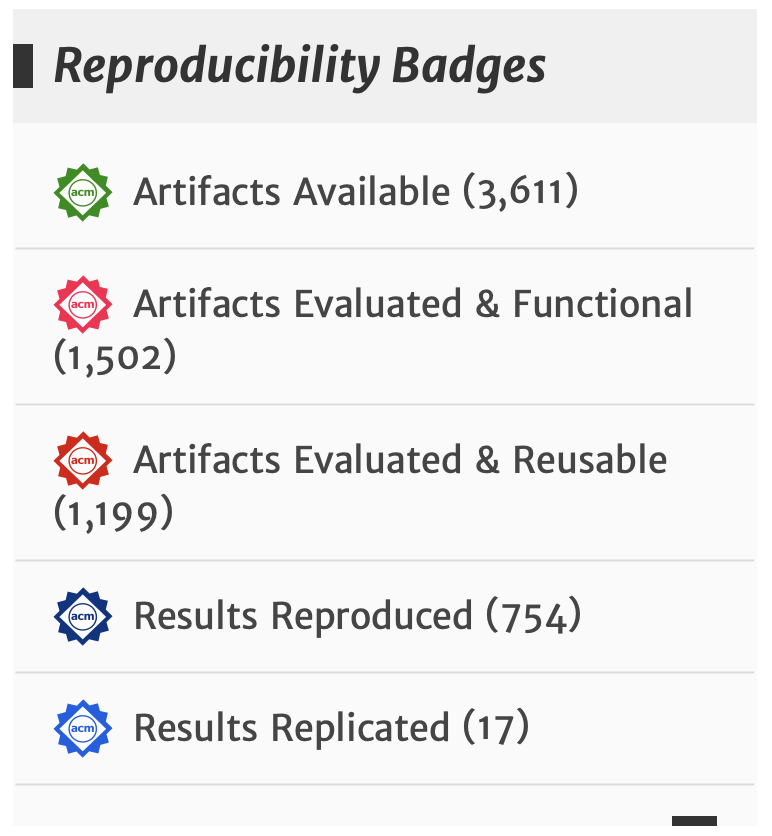
\includegraphics[scale=0.5]{acm_badges_5years-a} \\
    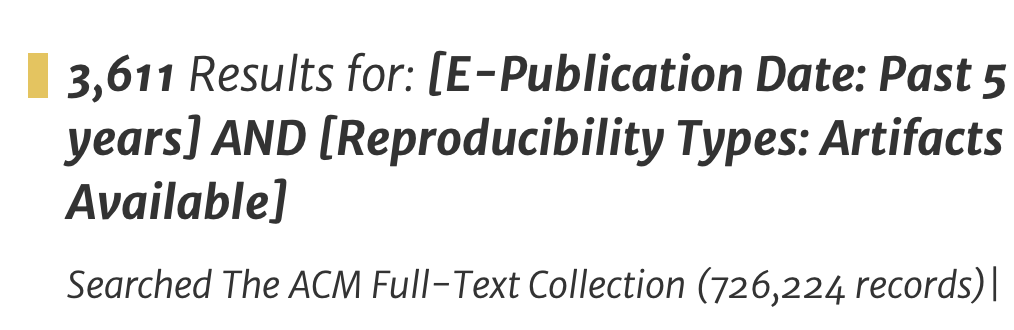
\includegraphics[scale=0.5]{acm_badges_5years-b} \\
    \caption{Results from a filter search in the ACM Digital Library for papers published in the past 5 years with an Artifacts Available badge.}
    \label{fig:acm_badges_5years}
\end{figure}




% These commands need to appear at the point where you want
% the first page to end.
\restoregeometry
\newgeometry{bottom=0.5in}

\section{Points of Agreement with the Article}
Lorem ipsum 


% 1. When figure position is crucial, use the [H] tag 
%    to enforce absolute positioning
% 2. Image files should be referenced without file extension
%\begin{figure}[H]
%    \centering
%    \includegraphics[scale=0.35]{iris_pairs} \\
%    \caption{This is an example figure}
%    \label{fig:my_label}
%\end{figure}


\subsection*{Disclosure Statement}
The authors have no conflicts of interest to declare.

%\subsection*{Acknowledgments}

 
%\subsection*{Contributions}



%Begin appendix section(s)
%\appendix

% Add appendices here:
%\section{Title}
%\label{appendix-customize-this-label}






% All references should be stored in the file "references.bib"
% Please do not modify anything below this line.
\printbibliography



\end{document}